
\documentclass[review,authoryear]{elsarticle}

\usepackage[utf8]{inputenc}
\usepackage{xcolor}
\usepackage{amsmath}

\usepackage{lineno}
    \linenumbers

\journal{Theoretical Population Biology}

\begin{document}

\begin{frontmatter}

\title{Allee Effect in Cultural Evolution}


\author[label1,label2]{Enrico R. Crema\corref{cor1}}
\cortext[cor1]{Corresponding Author: enrico.crema@upf.edu}
\author[label3]{Xavier Rubio-Campillo}

\address[label1]{CaSEs - Complexity and Socio-Ecological Dynamics Research Group, Universitat Pompeu Fabra, Barcelona}
\address[label2]{UCL Institute of Archaeology}
\address[label3]{CASE - Computer Applications in Science and Engineering, Barcelona Supercomputing Center}



\begin{abstract}
Several social learning strategies guide the selection of cultural variant through an evaluation of the expected benefits associated with each observed alternatives. The assumption of the social learner is that the payoff received by the transmitter, while displaying a given variant, is a proxy for  inferring the qualitative features of the variant itself. Here we explore the theoretical implications when: 1) the payoff attributed to a given cultural variant directly affects the reproductive success of its bearer;  and 2) payoff is density dependent, that is its expected amount is a function of the number of individuals possessing the same variant. We consider situations where such density dependence is both direct and inverse, with minimum and maximum critical thresholds bounding the range of positive payoff and a peak value at midpoint. This non-linear relationship, known as Allee effect, portrays a large number of behavioural traits that are enhanced by cooperation or mutual facilitation, but are constrained by finite amount of resources.  We explore the evolutionary dynamics of a single trait-two variants model, each exhibiting a different Allee effect. We use a modified Lotka-Volterra model of payoff-biased social learning, and show that different degrees of reliance on social learning can exhibit a variety of equilibria, including episodes of reversion, stable co-existence, and fixation.

\end{abstract}

\begin{keyword}
Social Learning\sep Cultural Evolution\sep Allee Effect\sep Cooperation\sep Carrying Capacity
\end{keyword}

\end{frontmatter}

\section{Introduction}

The last three decades have witnessed a steady growth of formal models of cultural evolution. Early works inspired by population biology \citep{cavallisforza_feldman_1981,boyd1985} have laid the foundation of a now mature trans-disciplinary field which unites the social and biological sciences \citep{mesoudi_etal_2006, mcelreath_and_boyd_2007}. The rich cross-fertilisation between different subfields has encouraged the designing of new analytical techniques as well as new uses for existing methods, but more crucially have prompted the development of theoretical models of how culture is acquired and transmitted between individuals~\citep{henrich_mcelreath2003,laland2004,mcelreath_and_boyd_2007,shennan_2009_patternprocess,Kempe_and_Mesoudi_2014,mesoudi_cultural_2015}. 

At the core of most models of social learning there is some heuristics that promotes the selection of a given cultural variant over another \citep{laland2004}. This can be based on some properties of the variant itself (\emph{content bias}) or derived from contextual cues (\emph{context bias}), such as the commonness or the rareness of a trait (\emph{conformist bias} and \emph{anti-conformist bias}), or  features associated with the transmitter such as prestige, success, or similarity to the learner (\emph{context bias}; see Henrich and McElreath \citeyear{henrich_mcelreath2003} for a review of these heuristics). 

This paper examines a group of social learning strategies generally referred to as \emph{payoff-based transmission} \citep{schlag1998,kendal_etal_2009,lake_and_crema_2012,baldini2013,kandler_and_laland_2013,crema_lake_inpress}. Here the probability of copying a cultural variant $i$ is directly proportional to a payoff $s$ exhibited by individuals possessing $i$. In other words the social learner assumes that the success of an individual (measured in $s$) is a function (of which details are often unknown) of the observed behavioural trait, that is $s=f(i)$. Several variants of this learning strategies have been proposed and explored, including: \emph{imitate the best}, where the social learner identifies and copies the trait possessed by the individual with the highest payoff; \emph{compare means}, where the social learner compare the average payoff of different strategies and chooses the highest; and the \emph{proportional imitation rule}, where the probability of adopting a variant is proportional to the difference in payoff between the demonstrator and the learner~\citep{schlag1998,baldini2013,crema_lake_inpress}. 

Whilst most studies focus on how difference in these imitation rules can drive the evolutionary dynamics of the cultural system, less attention has been given to the relationship between target traits and their payoff signals. Typically these are most likely some proxy of success (e.g. number of offspring, income, presence/absence of other traits associated with success or prestige, etc.)  that is assumed (by the social learner) to be correlated with intrinsic properties of the cultural variant. In most cases the causal link between  payoff and cultural trait is just inferred, and the exact processes and variables linking the two is unknown. Furthermore the strength of correlation between payoff and cultural trait can vary, introducing different degrees of uncertainty that can hinder the correct evaluation of a trait depending on the form of social learning. For example,~\citet{crema_lake_inpress} have shown that \emph{imitate the best} can even be detrimental in some situations where both payoff uncertainty  and the pool of potential social teachers are high.  This is because beneficial innovations are initially rare in a population, and hence even if their average payoff are higher than extant suboptimal alternatives, their probability of displaying the highest payoff, and hence being selected, is low.

The uncertainty in the payoff signal is derived by the presence of interacting cultural and physical traits, as well as the environment where the trait is expressed. Thus the function $s=f(i)$ should be better described as $s=f(i,\epsilon)$, where $\epsilon$ represent all additional hidden and latent variables that contribute, along with the cultural variant of interest $i$, to the payoff signal $s$. A trivial example is a fisherman who might evaluate the performance of a new hook (the target cultural trait) using as a cue the number of fish captured (the payoff signal). The correlation between the two is partly derived by the efficiency of the hook, but also by the rod, the choice of the bait, the amount of available prey, the choice of the fishing spot, the physical strength of the fisherman, and chance. In many cases we should expect that the social teacher and learner share many of these interacting traits as well as the environment where these are displayed. In other words, cultural and ecological inheritance should in part reduce the impact played by $\epsilon$, and consequently the uncertainty in the payoff-signal. There are however situations the payoff is highly variable even holding these variables constant. One of the most relevant examples are showcased in situations where the performance of a given  cultural variant $i$ is partly determined by the number of individuals $n_i$ expressing $i$ within a population. This \emph{density dependence}, which can be described by the payoff function $f(i,n_i)$, implies that the adoption (or abandonment) of a trait can alter its expected payoff-signal, potentially causing a cascade of feedback loops.  

Several behavioural traits are expected to show such a pattern. For example, behaviour linked to the exploitation of limited resources will exhibit a decline in payoff when density exceeds a critical threshold (i.e carrying capacity). In this case new optimal variants are likely to spread rapidly when they are rare, but as the number of individuals possessing them approach their respective carrying capacities, their beneficial effects will start to decline, the payoff will decrease, and eventually rarer suboptimal variants might be preferred (see Lake and Crema \citeyear{lake_and_crema_2012} for an extensive analysis). 

Density dependence does not necessarily imply only a negative correlation between population size and payoff. In many ecological contexts per-capita growth rate is positively correlated with population density, thus resulting into an inverse density dependence generally linked with processes such as cooperation, mutual facilitation, and environmental conditioning. This phenomena, known as \emph{Allee} effect \citep{allee1958,courchamp_etal_1999}, has been extensively studied  from both empirical and theoretical standpoints, and its consequences recognised in a wide variety of contexts, including habitat selection \citep{greene_and_stamps_2001}, resource competition \citep{jang2013},  dispersal \citep{steele_2009}, shifts in settlement pattern \citep{crema_2014}, colonisation events  \citep{kennet_etal_2006}, genetic diversity \citep{roques_etal_2012}, and extinction of languages \citep{sutherland_2003}. Yet, despite its ubiquity, we are unaware of any theoretical studies exploring how the simultaneous presence of direct and inverse density dependence in the payoff signal can affect the evolutionary dynamics of cultural transmission.   

Indeed, while the concept of Allee effect is well established in population ecology (see Kramer et al \citeyear{kramer_etal_2009} for a systematic review), there is no direct equivalent in the social sciences. Yet, there are multiple, established lines of evidence that support  the existence of both direct and inverse density dependence in human cultural and behavioural traits. For example several ethnographic studies on small scale societies show how the per-capita return of hunting groups show higher yield when the group size is not too small nor too big~ \citep{hill_and_hawkes_1983,janssen_and_hill_2014}. Other instances of inverse density dependence include population level activities such as the use of anthropogenic fire~\citep{bird2013} or selective hunting~\citep{dods_2002} which often require a population size above a certain critical density in order to promote sufficient niche enhancement and a consequent increase in payoff~\citep{rowley-conwy_and_layton_2011}. In a broader sense any cultural trait that benefits from direct or indirect cooperation, 
promote positive niche construction \citep{vandermeer_2008}, and requires a critical mass \citep{rogers_2003} are likely to exhibit some degree of Allee effect. The implication is thus not limited to traits that directly enhance reproductive fitness, and can include language~\citep{kandler2009}, organisational populations~\citep{caroll_and_hannan_1989} and communication technologies \citep{van_slyke_perceived_2007}.

Here we explore the broad consequences of the Allee effect by means of a theoretical equation-based model of cultural transmission. For the context of this study we narrow our scope by assuming that: 1) the social learning strategy is payoff-based; and 2)  the payoff is equivalent to the reproductive fitness of each individual. We demonstrate that direct and inverse density dependence can strongly affect the evolutionary trajectory of the system, leading to changes in the conditions required to reach specific equilibria, as well as to the emergence of unstable patterns characterised by temporary or permanent episodes of shifts between alternative cultural variants.

\section{The Model}
We consider the evolutionary dynamics of two mutually exclusive cultural variants which payoff functions are characterised by an Allee effect. We assume a non-fixed population of size $N$, subdivided into two subpopulations with sizes $a$ and $b$, each associated with a different cultural variant. We further assume that $a$ and $b$ can change as a result of intrinsic population growth/decline as well as shifts from one to the other as a result of cultural transmission. The core model can be depicted with the following coupled difference equation \eqref{eq1}:

\begin{equation}
\begin{aligned}
a_{t+1}& = a_t + a_t R_{a,t} + C_{a,b,t} \\
b_{t+1}& = b_t + b_t R_{b,t} + C_{a,b,t}
\label{eq1}
\end{aligned}
\end{equation}

where $a_{t+1}$ and $b_{t+1}$ are the population sizes of each variant at time $t+1$. This is given by the number of individuals during the previous time-step ($a_t$ and $b_t$), the reproductive rate of each population ($R_{a,t}$ and $R_{b,t}$), and the shift from one population to another as a result of cultural transmission ($C_{a,b,t}$).

The reproductive growth rate $R$ of each population is defined by the following pair of equations:

\begin{equation}
\begin{aligned}
R_{a,t}& = r_a \left(\frac{a_t}{A_a}-1\right)\left(1-\frac{a_t}{K_a}\right)\\
R_{b,t}& = r_b \left(\frac{b_t}{A_b}-1\right)\left(1-\frac{b_t}{K_b}\right) 
\label{eq2}
\end{aligned}
\end{equation}

where $r$ is the basic growth rate, $A$ is the critical density and $K$ is the carrying capacity, following the condition $0<A < K$. Notice that here $R$ is also the payoff of each variant for a given population size.  

Equation \eqref{eq2} depicts the so called \emph{strong} Allee effect \citep{Wang_and_Kot_2001}, where reproductive rate is negative when population density is either below $A$ or above $K$, and in this case reach its maxima $R_{max}=\frac{r(A-K)^2}{4AK}$ when density is equal to $\frac{(K-A)}{2}$. 

The cultural transmission component of equation \eqref{eq1} is based on the \emph{proportional imitation rule} \citep{schlag1998}. In this case, the probability of an individual with lower payoff to adopt the alternative, optimal variant is proportional to the difference in the growth rates. This is formally portrayed as follows:

\begin{equation}
\begin{aligned}
\label{eq3}
C_{a,b,t} = 
\begin{cases}
0& \text{if } R_{a,t} = R_{b,t}\\
\zeta(a_t+a_tR_{a,t})& \text{if } R_{a,t} > R_{b,t}\\
-\zeta(b_t+b_tR_{b,t})& \text{if } R_{a,t} < R_{b,t}
\end{cases}
\end{aligned}
\end{equation}

where $\zeta$ defines the proportion of individuals changing strategy, and given by \eqref{eq4}:

\begin{equation}
\begin{aligned}
\label{eq4}
\zeta = 
\begin{cases}
z& \text{if }|R_{a,t}-R_{b,t}| > m\Delta\\
z\frac{|R_{a,t}-R{b,t}|}{m\Delta}& \text{if }|R_{a,t}-R_{b,t}| \leq m\Delta\\
\end{cases}
\end{aligned}
\end{equation}

where $z$ is a measure of reliance in social learning (effectively equivalent to highest possible transmission rate), $\Delta$ is the maximum between $R_{max(a,t)}$ and $R_{max(b,t)}$, and $m$ is a calibration parameter that measures the perception of the difference in the payoffs (i.e. small values of $m$ determines a higher rate by which the theoretical maximum transmission rate is reached), thus portraying also potential acquisition costs of the new variant (c.f. "threshold of evidence', Henrich, \citeyear{henrich2001cultural}: 994)

\section{Results}

We investigate the equilibrium conditions for different initial population sizes of $a$ and $b$ and different settings of $z$, $A$, and $K$, ensuring that in all cases $K_b \geq K_a$. We assumed that two strategies differed only in their critical densities and carrying capacities but not on their intrinsic payoffs. To achieve this we set $r_b=\rho r_a$, where $\rho$ is a constant\footnote{Given two variants with the same baseline growth rate (i.e. $r_a=r_b$), equation \eqref{eq2} returns a lower $R$ for the variant with higher $A$ and $K$. In order to avoid this we increased the baseline of the strategy with lower $R$ by a factor $\rho$, given by the following equation:
\begin{align*}
\rho=\frac{A_bK_b(K_a-A_a)^2}{A_aK_a(A_b-K_b)^2}
\end{align*}
  } 
that ensures that the two variants have always the same $R_{max}$. Given that equations \ref{eq1}-\ref{eq4} have no analytical solution that we are aware of, we identified equilibrium conditions via simulation (examples codes are provided on the ESM).

\subsection{Equilibrium conditions without social learning}

When $z=0$, equations \ref{eq1}-\ref{eq4} becomes a standard cubic growth model with Allee effect, where the success (or failure) of a given focal trait is primarily given by its own density. For a generic cultural trait $x$, the model predicts three equilibrium points at $x=0$ (extinction), $x=A_x$, and $x=K_x$. The equilibrium $x=A_x$ is unstable for all values of $r_x$, whereas the stability of the node at $x=K_x$ is a function of the per-capita growth rate $r_x$. Increasing the latter decreases the stability of fixed points~\citep{scheuring_1999}, leading to the transition from point attractors (with equilibrium at $x=K_x$), to limit cycles and chaotic dynamics with islands of stability (see fig. \ref{fig:bifurcationDiagram}). 

\begin{figure}[h!]
  \centering
      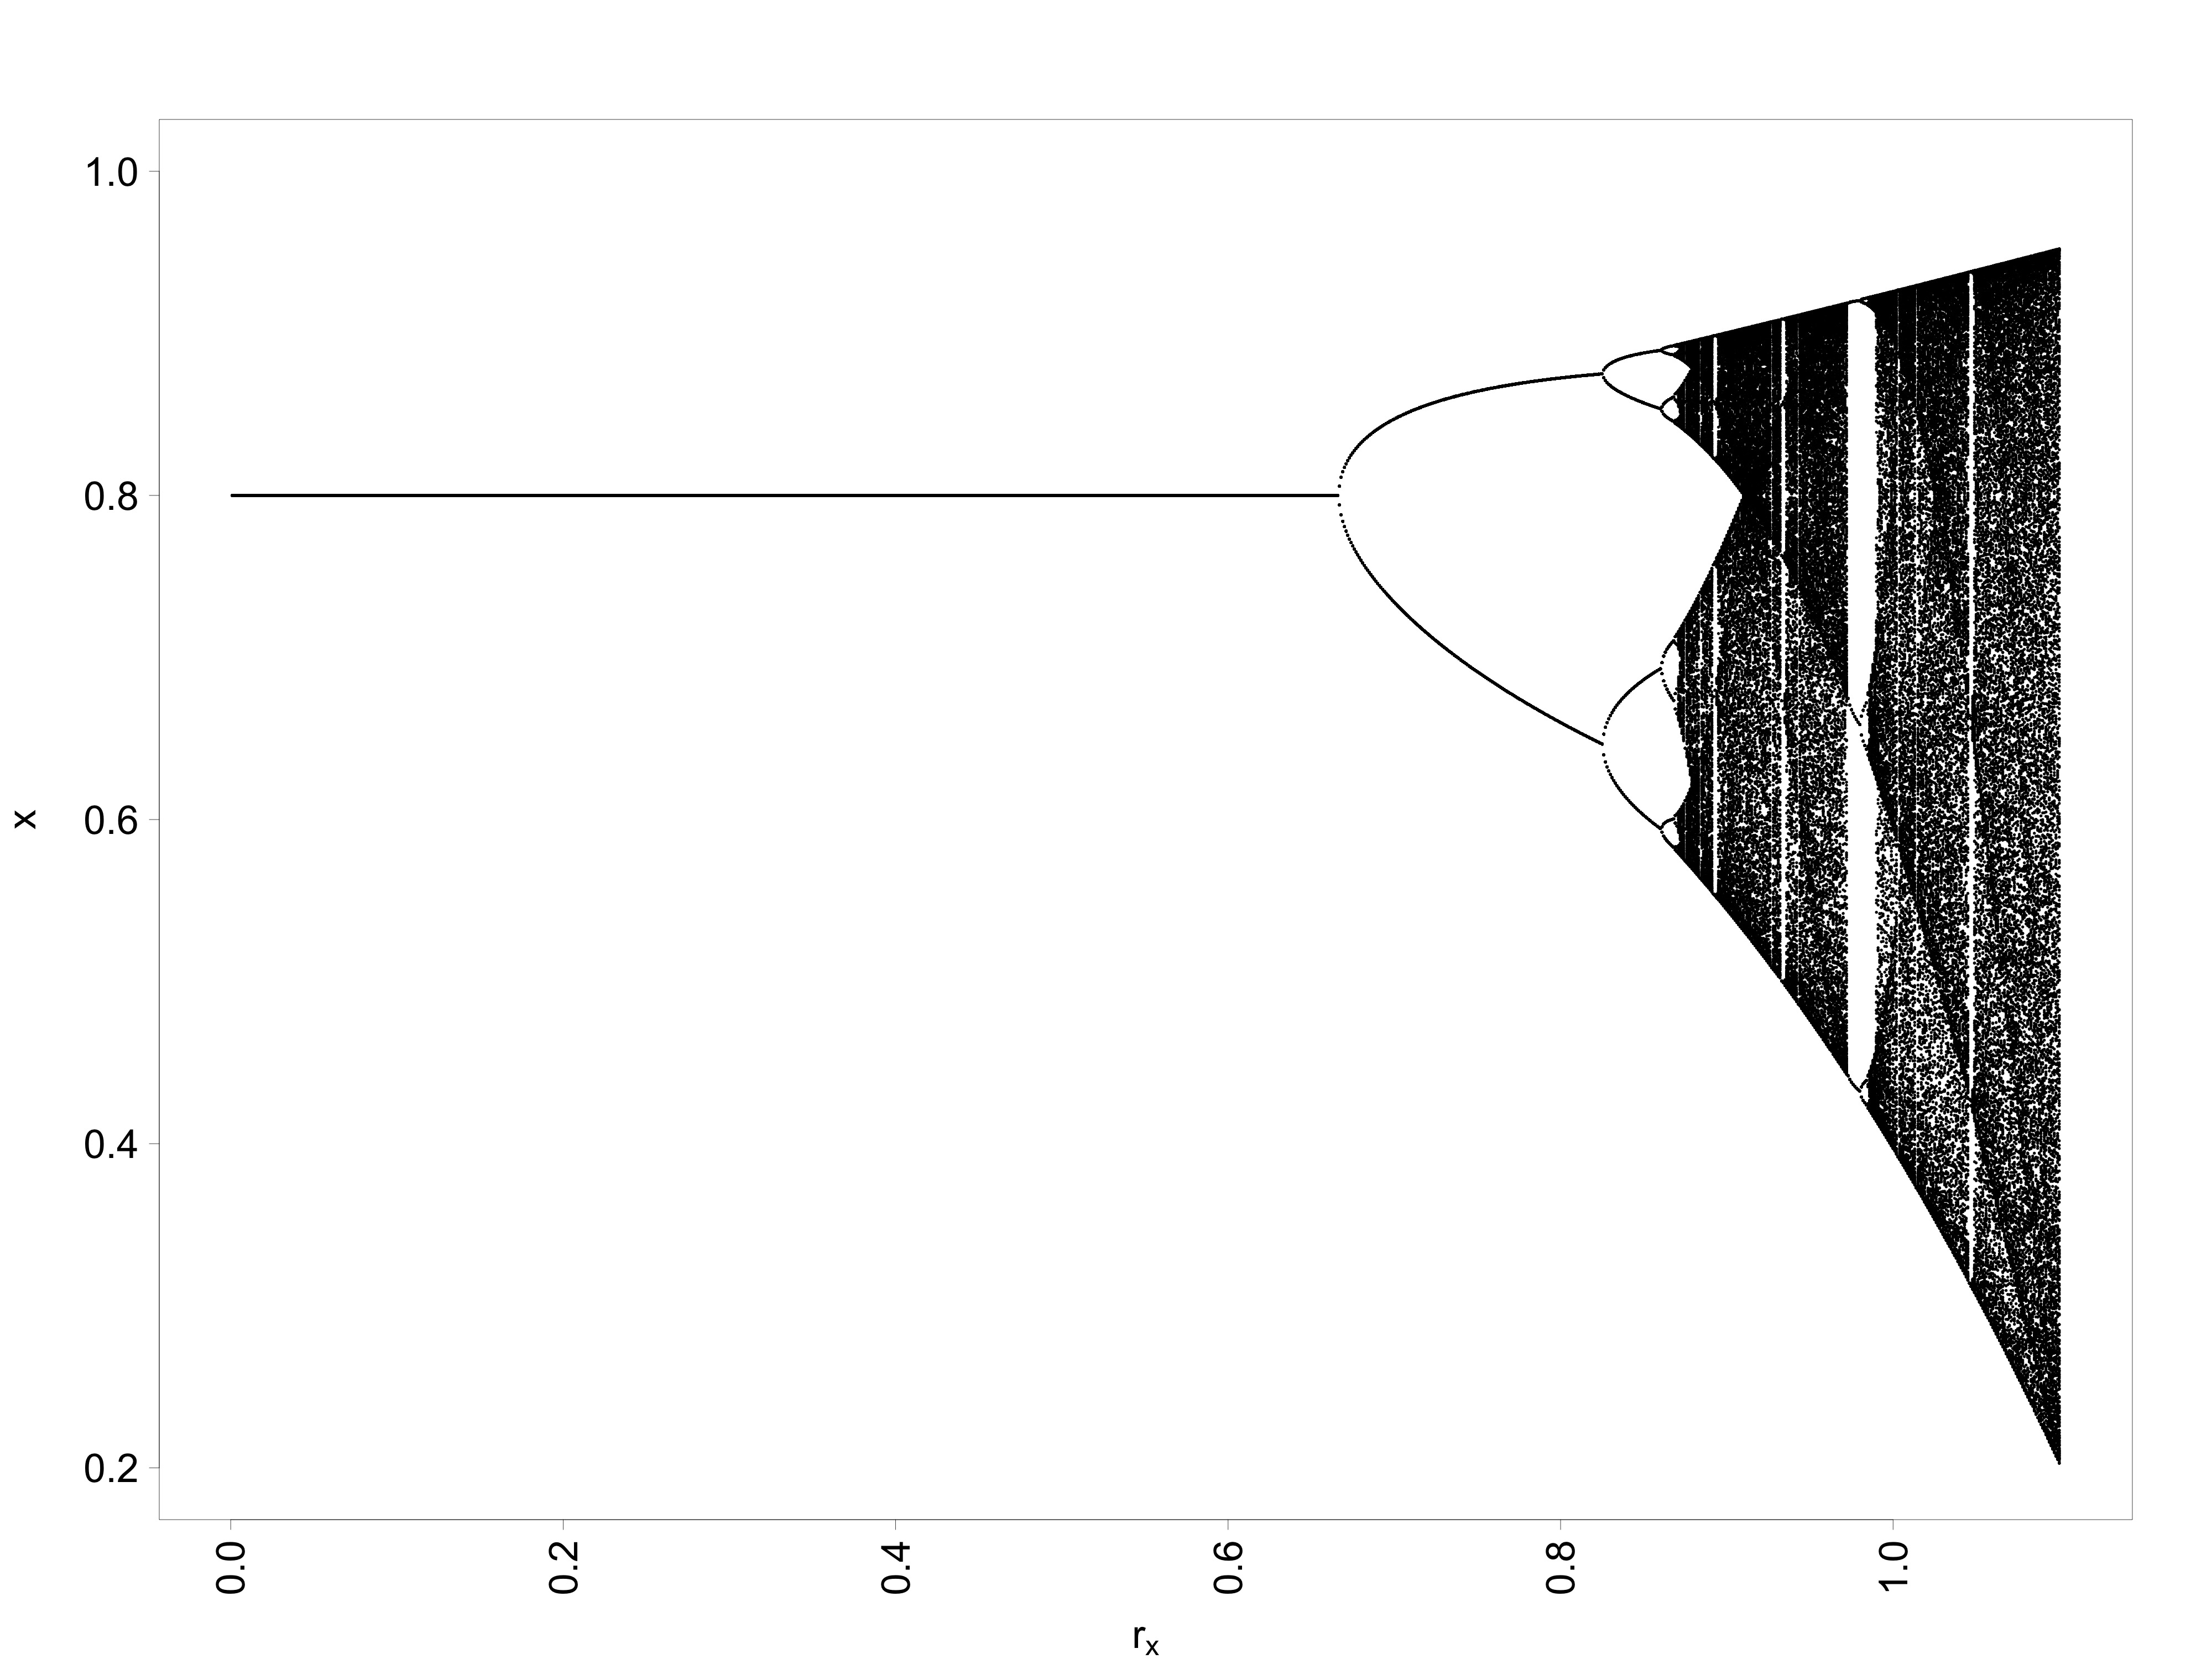
\includegraphics[width=1\textwidth]{./figures/figure1.jpg}
  \caption{Bifurcation diagram of a single population model with $A_x=0.2$ and $K_x=0.8$. For $0<r_x<0.6649747$, any initial value of $x$ greater than $A_x$ converges to $K_x$.}
    \label{fig:bifurcationDiagram}
\end{figure}

For the rest of the paper we will consider only scenarios where the node $x=K_x$ is stable when $z=0$. In this case the initial value of $x_{t=0}$ will determine the ultimate equilibria of the system: extinction, if $x_{t=0}<A_x$; unstable equilibrium, if $x_{t=0}=A_x$; and stable equilibrium, if $x_{t=0}>A_x$. Thus in a 2-trait model, the coexistence of both variants is guaranteed only when the initial density of both traits are above their respective critical densities, otherwise we should expect that either (i.e. $a_{t=0} \geq A_a$ and $b_{t=0}<A_b$ or $a_{t=0}<A_a$ and $b_{t=0} \geq A_b$) or both (i.e. when $a_{t=0}<A_a$ and $b_{t=0}<A_b$) variants are ultimately extinct (see fig. \ref{fig:NoTransmissionBasin}). 

\begin{figure}[h!]
  \centering
      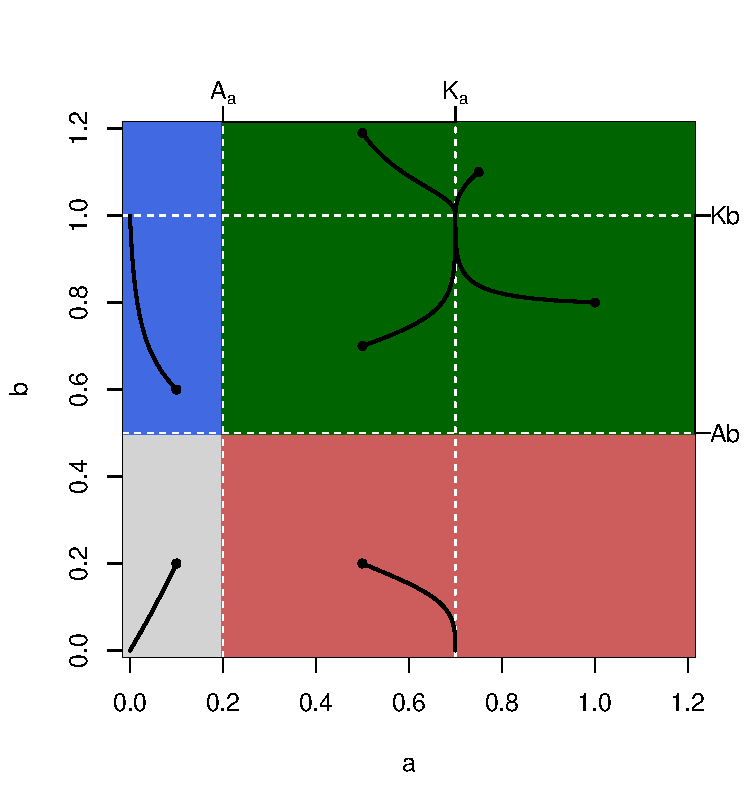
\includegraphics[width=1\textwidth]{./figures/figure2.pdf}
  \caption{Basins of attraction for the four equilibria (mutual extinction: grey; extinction of $a$: blue; extinction of $b$: red; stable coexistence: green). Solid lines represent trajectories of the system for different initial conditions, represented by dots. Model parameters: $A_a=0.2$; $K_a=0.7$; $A_b=0.5$; $K_b=1.0$; $r_a=r_b=0.05$}.
    \label{fig:NoTransmissionBasin}
\end{figure}

\subsection{Effects of social learning}

When social learning is enabled (i.e. when $z>0$), the stability of the nodes are perturbed by individuals switching from one strategy to another, leading to two major changes in the equilibrium properties of the system. 

First, the basins of attraction are transformed, and hence the system equilibrium at $z=0$ and $z>0$ can be different for the same initial conditions. This is particularly the case for combinations of $a$ and $b$ that are closer to the boundaries between two or more basins when $z=0$.  Figure \ref{fig:TransmissionBasin} shows an example of this. When social learning is not present (fig.~\ref{fig:TransmissionBasin} left), the initial conditions $i$, $j$, and $k$ result into a stable equilibrium at $a=K_a$ and $b=K_b$, whilst the starting point $l$ leads to the extinction of $b$. When $z=0.05$ (fig.~\ref{fig:TransmissionBasin} right), the basins of attractions are modified, resulting into different trajectories and in some cases different equilibria for the same initial conditions. Thus $i$ and $k$ are no longer leading to the coexistence of both traits but to the demise of one or the other, whilst $l$ now ensures the coexistence of both variants. 

\begin{figure*}
  \centering
      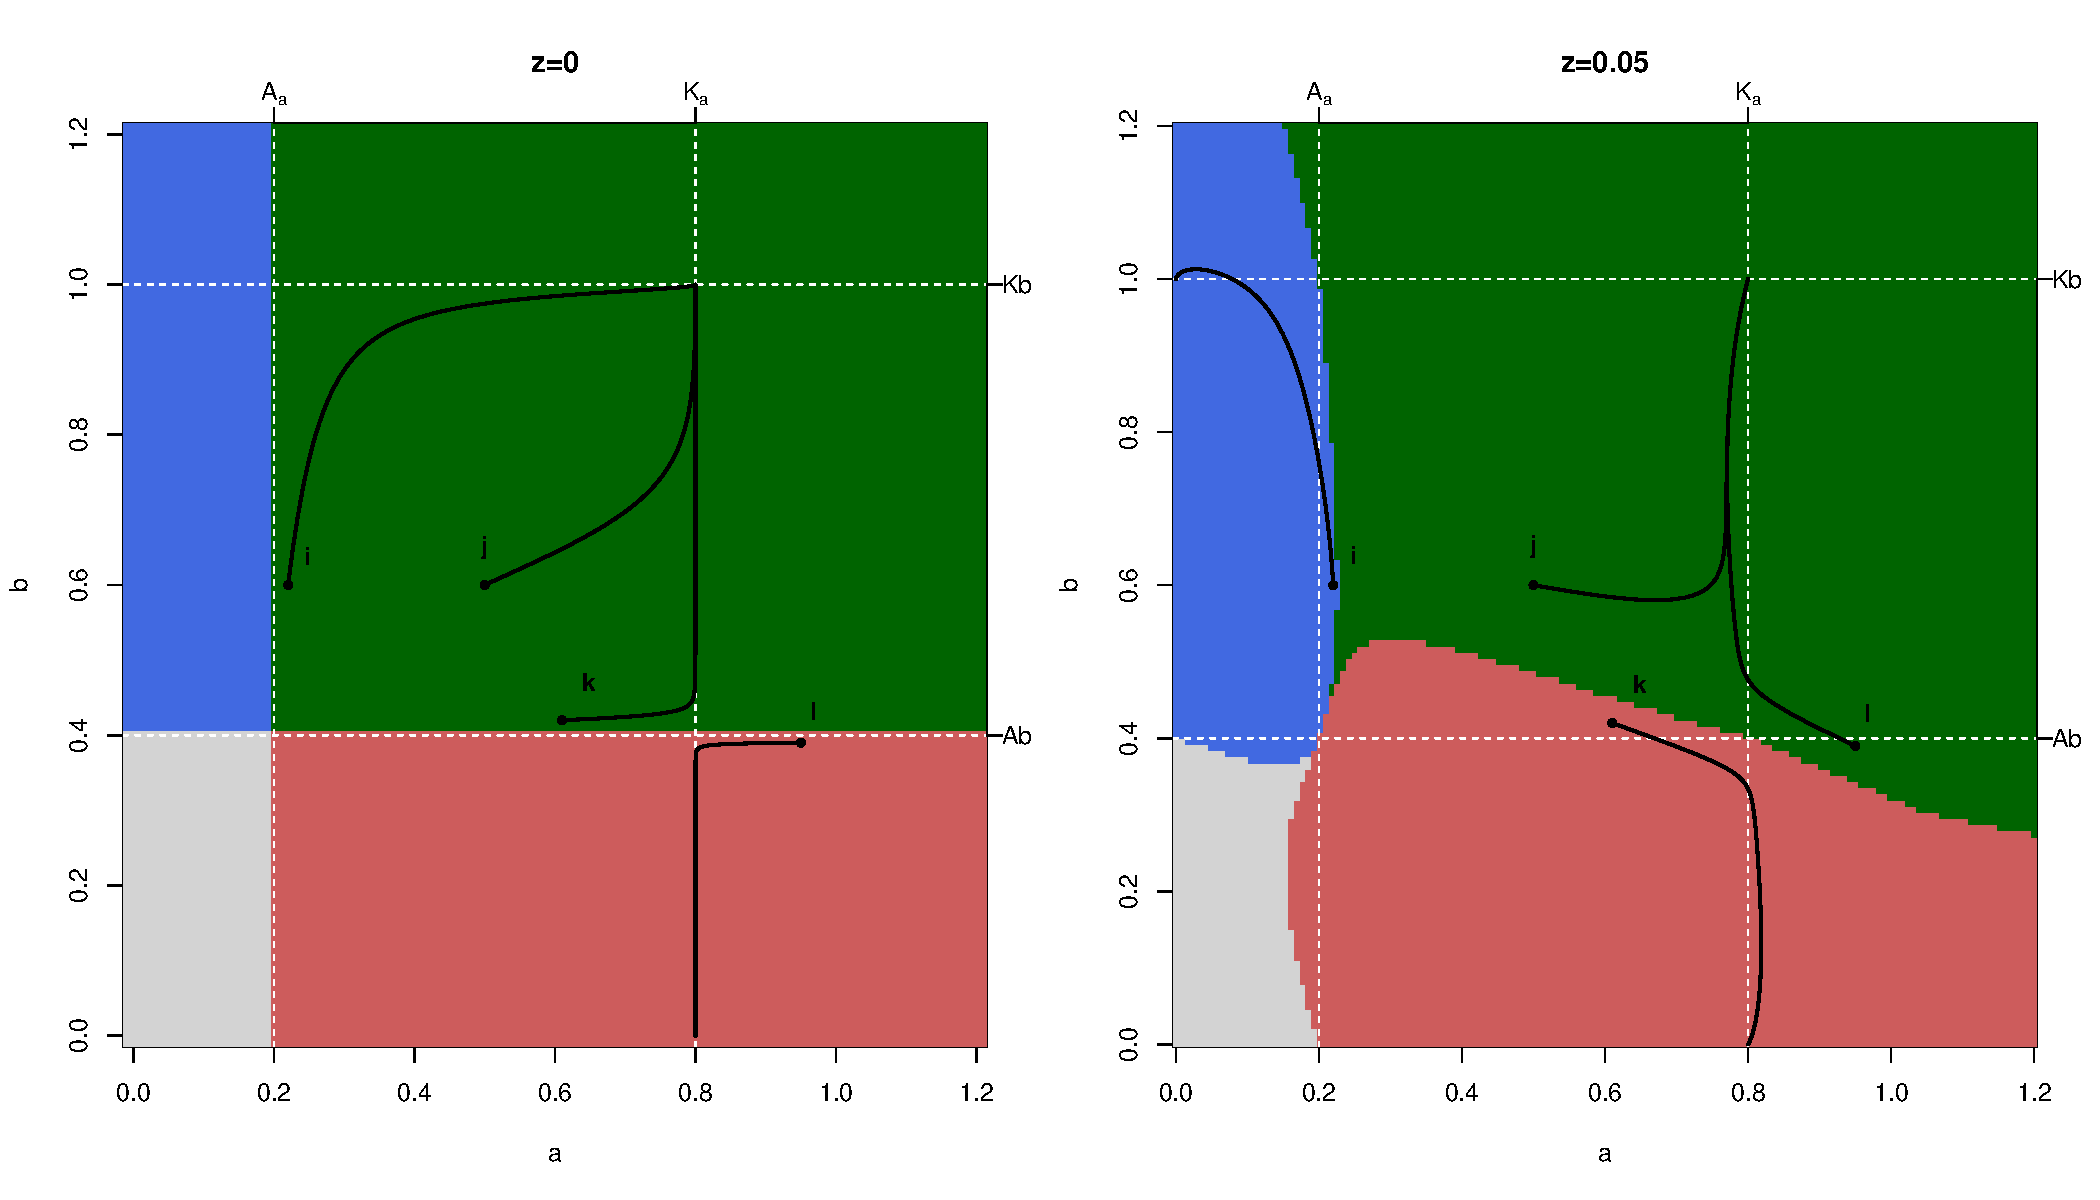
\includegraphics[width=\columnwidth]{./figures/figure3.pdf}
  \caption{Basins of attraction for the four equilibria (mutual extinction: grey; extinction of $a$: blue; extinction of $b$: red; stable coexistence: green) with (right) and without (left) social learning. Model parameters: $A_a=0.2$; $K_a=0.8$; $A_b=0.35$; $K_b=0.95$; $r_a=0.05$; $r_b=0.1039063$; $z=0$ (left panel) and $z=0.2$ (right panel) } 
    \label{fig:TransmissionBasin}
\end{figure*}


Second, when the magnitude of social learning is high, the system is subject to effects similar to those observed with an increase in the per-capita growth rate $r$ (cf. fig. \ref{fig:bifurcationDiagram}), that is a decrease in the stability of the fixed points. Figure \ref{fig:TSsocialLearning} shows fluctuations in population size of the system over time for different values of $z$. Here low values of $z$ do not change the equilibrium point at ($a=K_a$ and $b=K_b$). However, at $z \geq 0.6$ unstable dynamics can be observed leading the system towards limit cycles. In this configuration the regulatory effect of negative fitness is minimised by the fast rates of cultural transmission (i.e. individuals switch to the alternative trait before the decrease in payoff lead to a population decline).

\begin{figure}
  \centering
      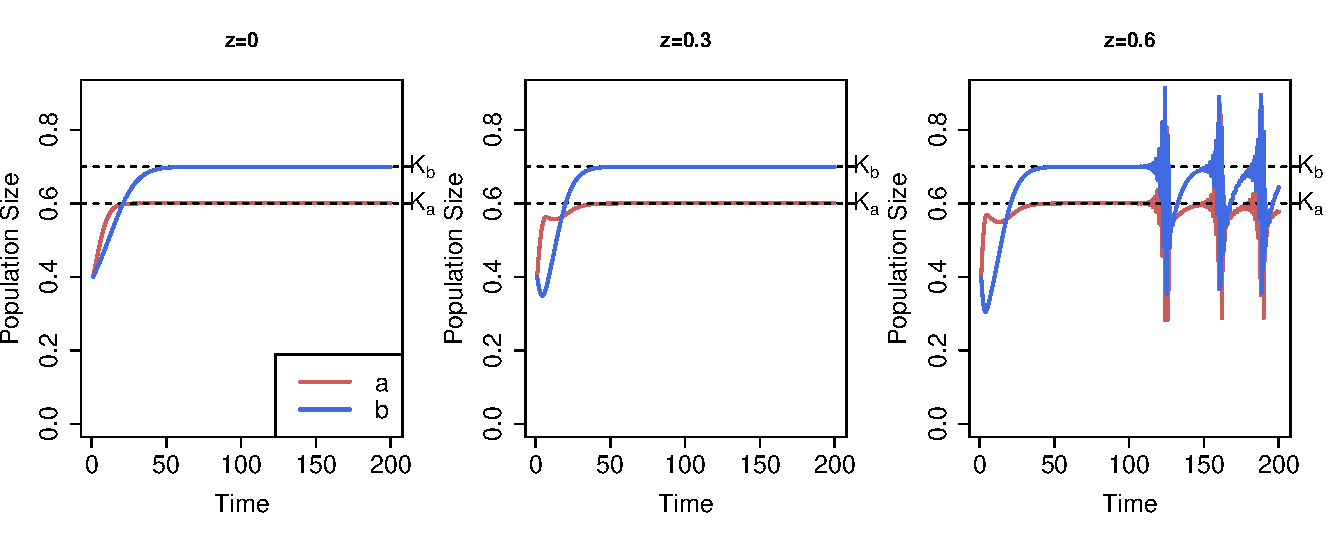
\includegraphics[width=1\textwidth]{./figures/figure4b.pdf}
  \caption{Time series of population size for $z=0$ (left), $z=0.3$ (center) and $z=0.6$ (right). Increasing values of $z$ shift the system from the co-existence equilibrium towards a limit cycle with abrupt population changes. Model parameters: $A_a=0.1$; $A_b=0.2$; $K_a=0.6$; $K_b=0.7$; $r_a=r_b=0.05$}
    \label{fig:TSsocialLearning}
\end{figure}

\subsection{Differences in critical density and carrying capacities}

The analyses of the previous section suggest that the number of individuals engaging into social learning within a given temporal interval can have major impacts in the qualitative state of the final equilibrium (c.f. fig. \ref{fig:TransmissionBasin}). This number is dependent on the propensity to engage into cultural transmission ($z$) and the potential difference in the payoff of the two available cultural variants. The latter can be determined by difference in the baseline reproductive rate ($r$), but also by the degree of overlap in the range of positive payoff for the two variants ($[A_a,K_s]$ and $[A_b,K_b]$) alone. We explore this second scenario and its relationship to $z$ using the following constraints for our parameters:

\begin{equation}
\begin{aligned}
\label{eqOverlap}
A_b = A_a + (1-\lambda)(K_a-A_a)\\
K_b = K_a + (1-\lambda)(K_a-A_a)
\end{aligned}
\end{equation}

Equation \eqref{eqOverlap} ensures that the difference between carrying capacity and critical density is hold constant and equal between the two variants, so that the parameter $\lambda$ can be interpreted as an inverse  measure of overlap: when $\lambda=1$ the two variants are identical, and when $\lambda=0$, the critical density of one strategy becomes equal to the carrying capacity of the other (i.e. $A_b=K_a$). Figure \ref{fig:overlap} examines three different settings of $\lambda$  with low ($z=0.05$) and intermediate ($z=0.2$) degrees of reliance on social learning. The plot suggests that, higher values of $z$ limits the number of initial conditions where a stable co-existence is achieved within the positive payoff zone (i.e. when the initial conditions for $a$ and $b$ are within the intervals $[A_a,K_a]$ and $[A_b,K_b]$), although the magnitude of this effect is smaller for lower values of $\lambda$ (i.e. smaller overlap). We can further investigate this point by computing the relative areas of different basins of attraction within the positive payoff zone for different parameter combinations of $z$ and $\lambda$. The results (fig. \ref{fig:percentages}) confirms that indeed with high overlap and high rates of social learning conditions enabling the stable coexistence is reduced, initially as a result of an increase of conditions promoting the dominance of one variant, and eventually because the unstable fluctuations regime takes over. When  $\lambda$ is small, this pattern disappears, and the relationship between $z$ and the size of the basin of attraction for stable coexistence becomes more or less stable for each value of $\lambda$. 

\begin{figure*}
  \centering
      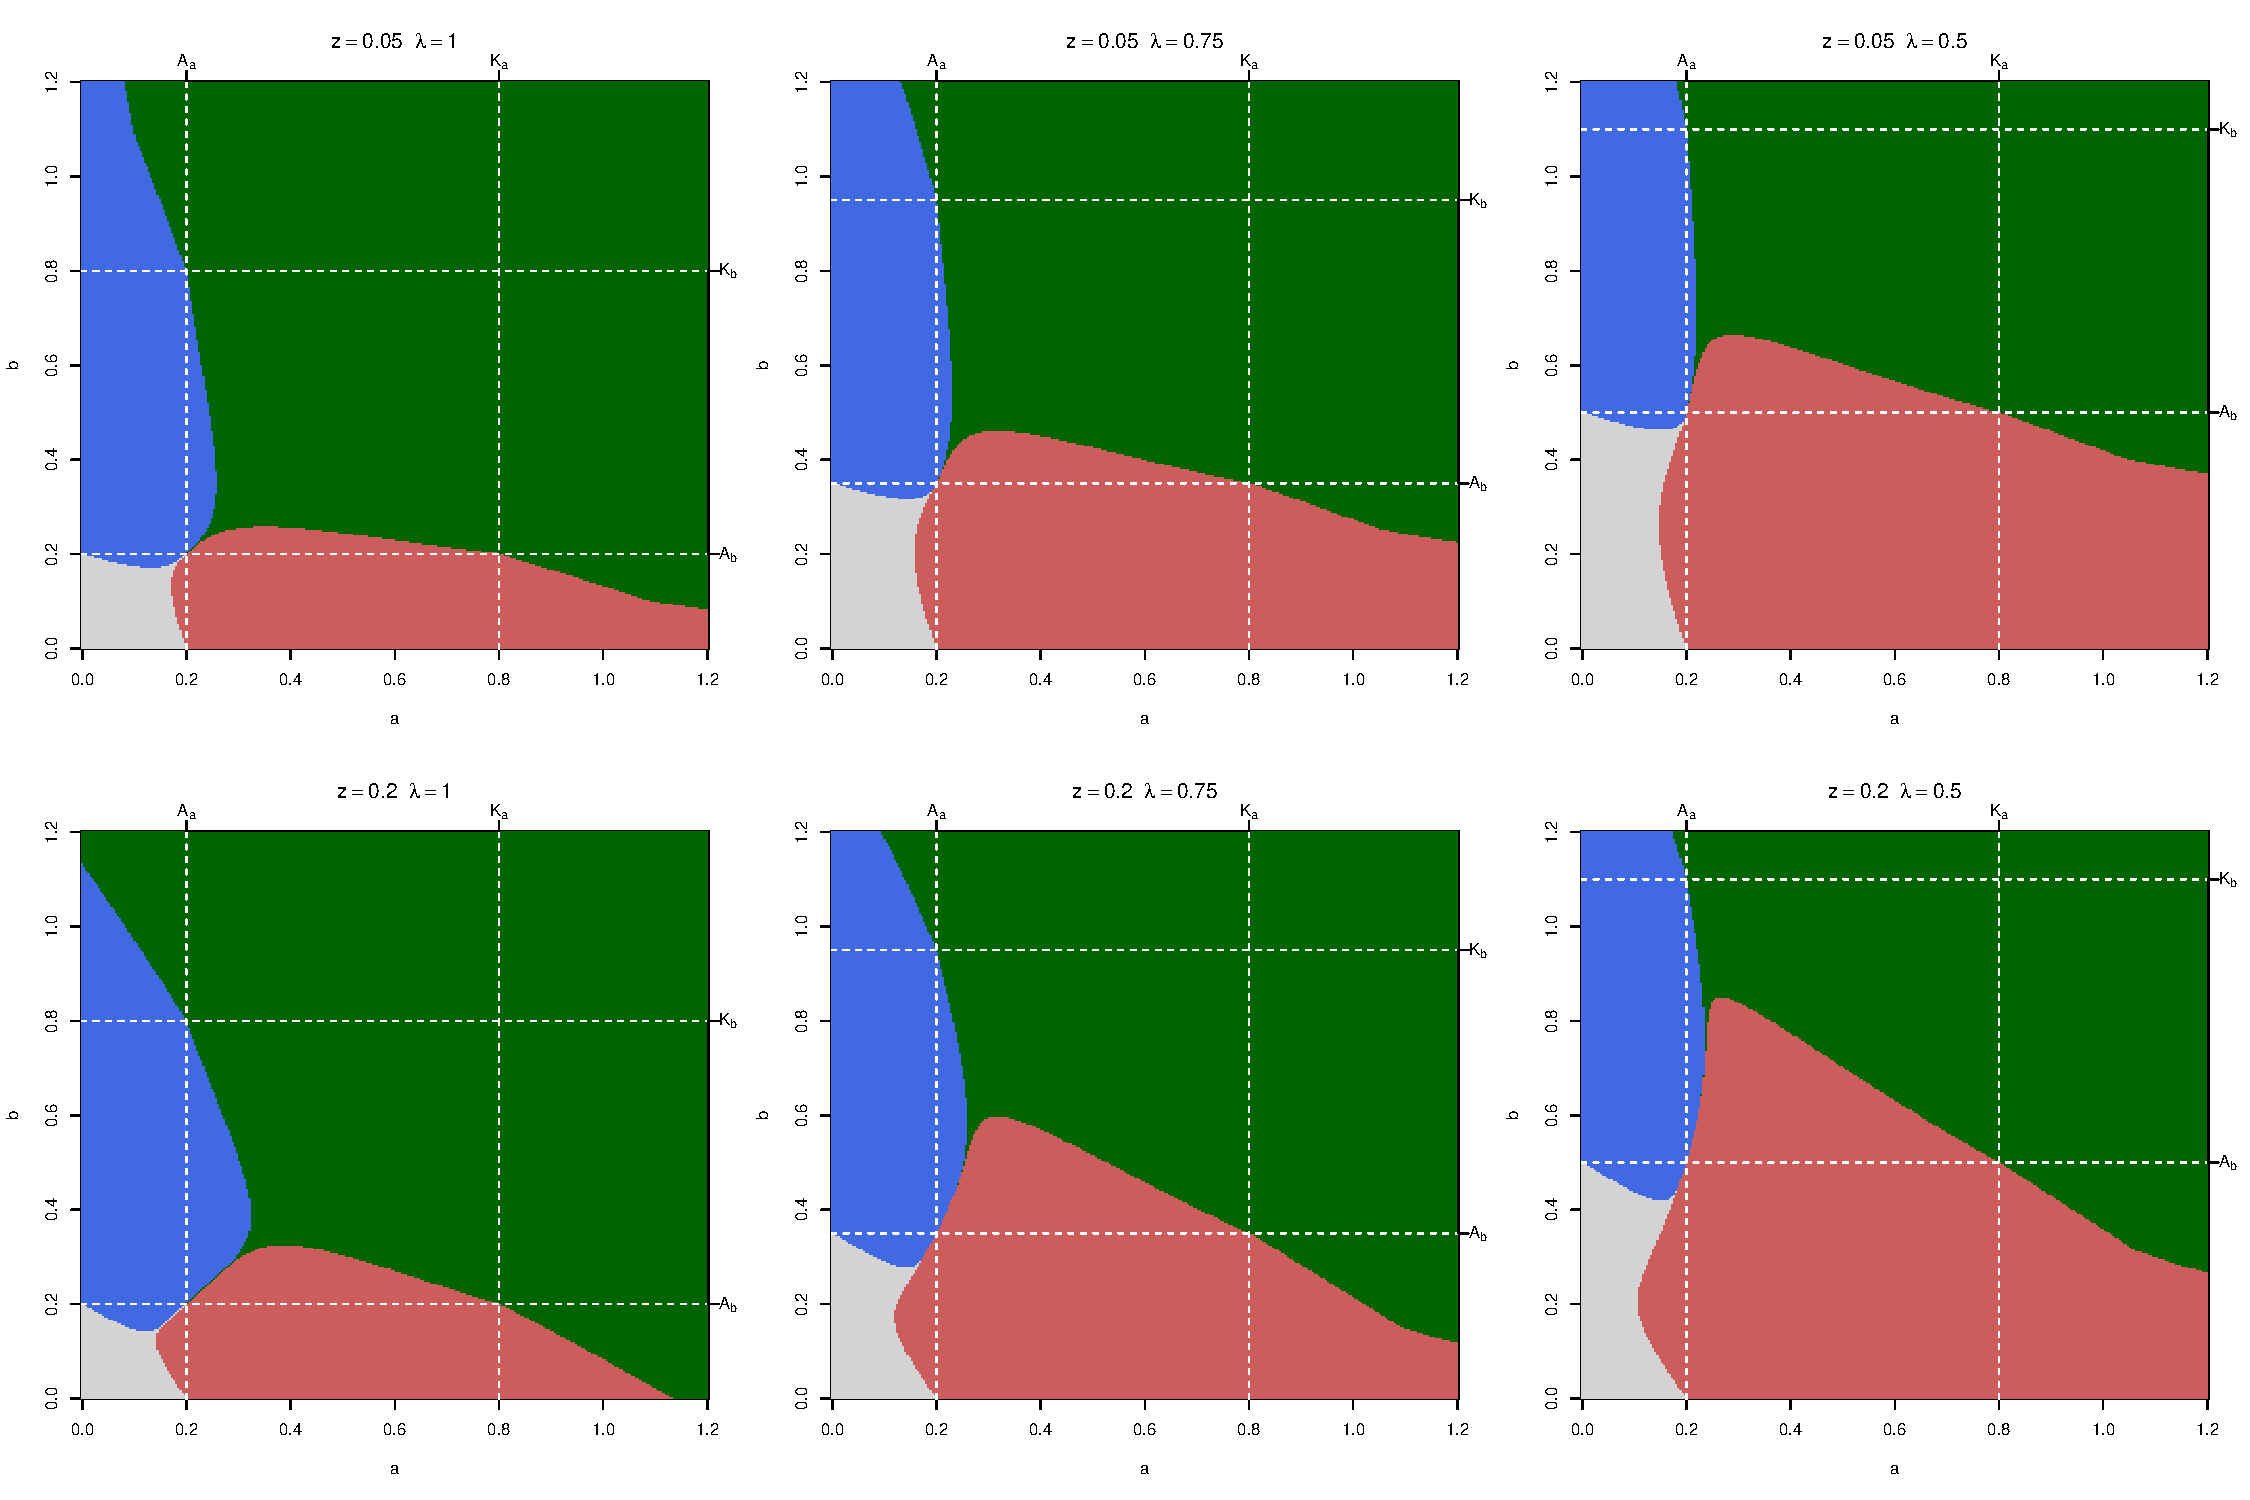
\includegraphics[width=\textwidth]{./figures/figure5}
  \caption{Basins of attraction for $z=0.05$ (top) and $z=0.2$ (bottom); $\lambda=1$ (left), $\lambda=0.75$ (middle) and $\lambda=0.5$ (right)}
    \label{fig:overlap}
\end{figure*}

\begin{figure}
  \centering
      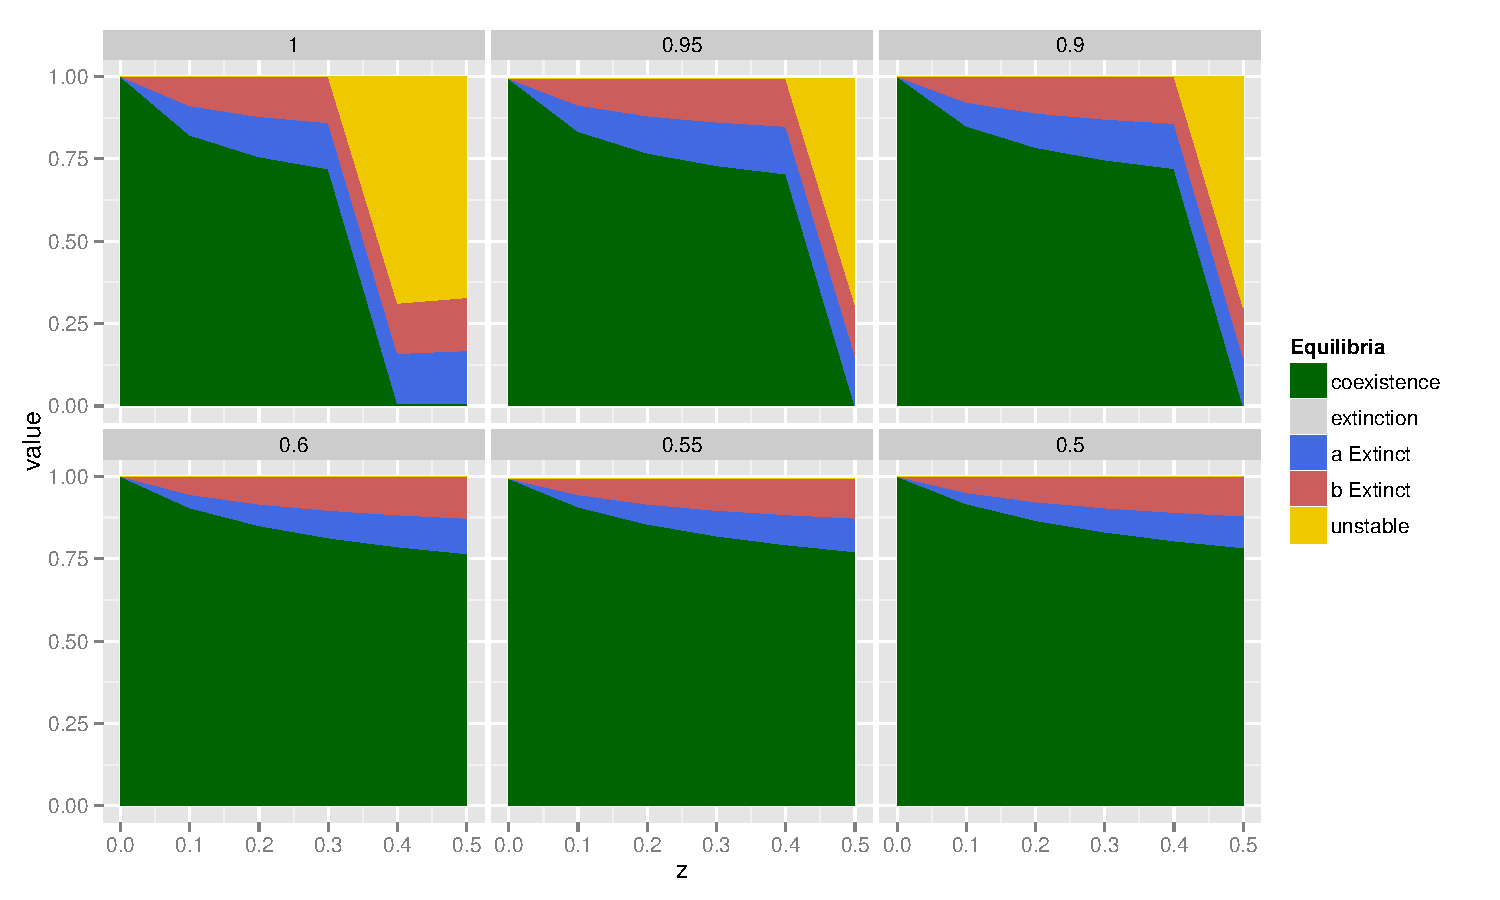
\includegraphics[width=\textwidth]{./figures/figure6}
  \caption{Proportion of initial conditions falling in each basin of attraction for different values of $\lambda$. X axis controls the parameter $z$ defining social learning. Model parameters: $A_a=0.2$; $K_a=0.8$; $r_a=0.05$}
    \label{fig:percentages}
\end{figure}

\subsection{Effect of competition}

The results detailed in previous section indicates that, within the positive payoff region, fixation to one strategy or another can occur only for a comparatively narrow set of initial conditions close to the boundaries between different basins of attractions. For all other conditions we expect to observe either a stable coexistence or unstable fluctuations depending on the propensity on social learning and the ease by which a switch from one variant to another is possible. The results thus implies that if two variants have similar payoff values, there is no intrinsic advantage of one strategy over the other. Thus the variant with higher critical thresholds $A$ and $K$ do not necessarily predominate over a wider range of initial population sizes, and instead its full adoption by the entire population $N$ is ensured only when its initial density is comparatively high (e.g. above or equal its maximum payoff) and when the alternative strategy is close to its critical threshold $A$. This also implies that if the variant with higher $A$ and $K$ is novel, some mechanism (e.g. an alternative form of social learning) must ensure that its density approaches its highest payoff, and at the same, the incumbent strategy should exhibit a comparatively low density. Alternatively, the novel variant should either exhibit a higher payoff (thus has some intrinsic advantage) or some form of competition between the two variant should be considered. Here we briefly explore the latter scenario, by relaxing the assumption of independence in the computation of the payoff of each variant. For instance many subsistence strategies do not have fully independent resource pools, and hence the success of a given variant might be detrimental to the payoff of the other irregardless of the effects provoked by cultural transmission. We can revise our core model by including new terms portraying the competition effect between the two resources:  

\begin{equation}
\begin{aligned}
R_{a,t}& = r_a \left(\frac{a_t-c_{A_a}b_t}{A_a}-1\right)\left(1-\frac{a_t-c_{K_a}b_t}{K_a}\right)\\
R_{b,t}& = r_b  \left(\frac{b_t-c_{A_b}a_t}{A_b}-1\right)\left(1-\frac{b_t-c_{K_b}a_t}{K_b}\right) 
\label{eqCompetition}
\end{aligned}
\end{equation}

where the four new parameters $c_{A_a}$, $c_{A_b}$, $c_{K_a}$ and $c_{K_b}$, measure respectively the negative (or positive) effect determined by the number of individuals of the other variant. 
When $c_{A}>0$ the Allee threshold is essentially increased, while when $c_{K}>0$ the carrying capacity is diminished as function of the other population. 
Larger values of any of the $c$ parameters dictates a stronger influence of the other population. While the unstable node at the critical density ($A$) is maintained, equation \eqref{eqCompetition} does not have an equilibrium point at carrying capacity. Instead a new, competition-driven equilibrium can be identified by the following pair of equations: 

\begin{equation}
\begin{aligned}
a=\frac{K_a-c_{K_b}K_b}{1-c_{K_b}c_{K_a}}\\
b=\frac{c_{K_a}K_a-K_b}{c_{K_a}c_{K_b}-1}
\label{eqCompetitionSolution}
\end{aligned}
\end{equation}

Notice that when all competition parameters are set to 0, equation \eqref{eqCompetitionSolution} points to $K_a$ and $K_b$ as the stable equilibrium node. 

Figure \ref{fig:competition} shows a scenario where strategy $a$ is dominant over strategy $b$. Here the combination of high reliance on social learning and competitive advantage can have a drastic effect to the system, with a wide combination of parameters leading to a fixation to $b$, and a stable coexistence ensured only for when $a$ has densities close to its carrying capacity.

\begin{figure*}[h!]
  \centering
      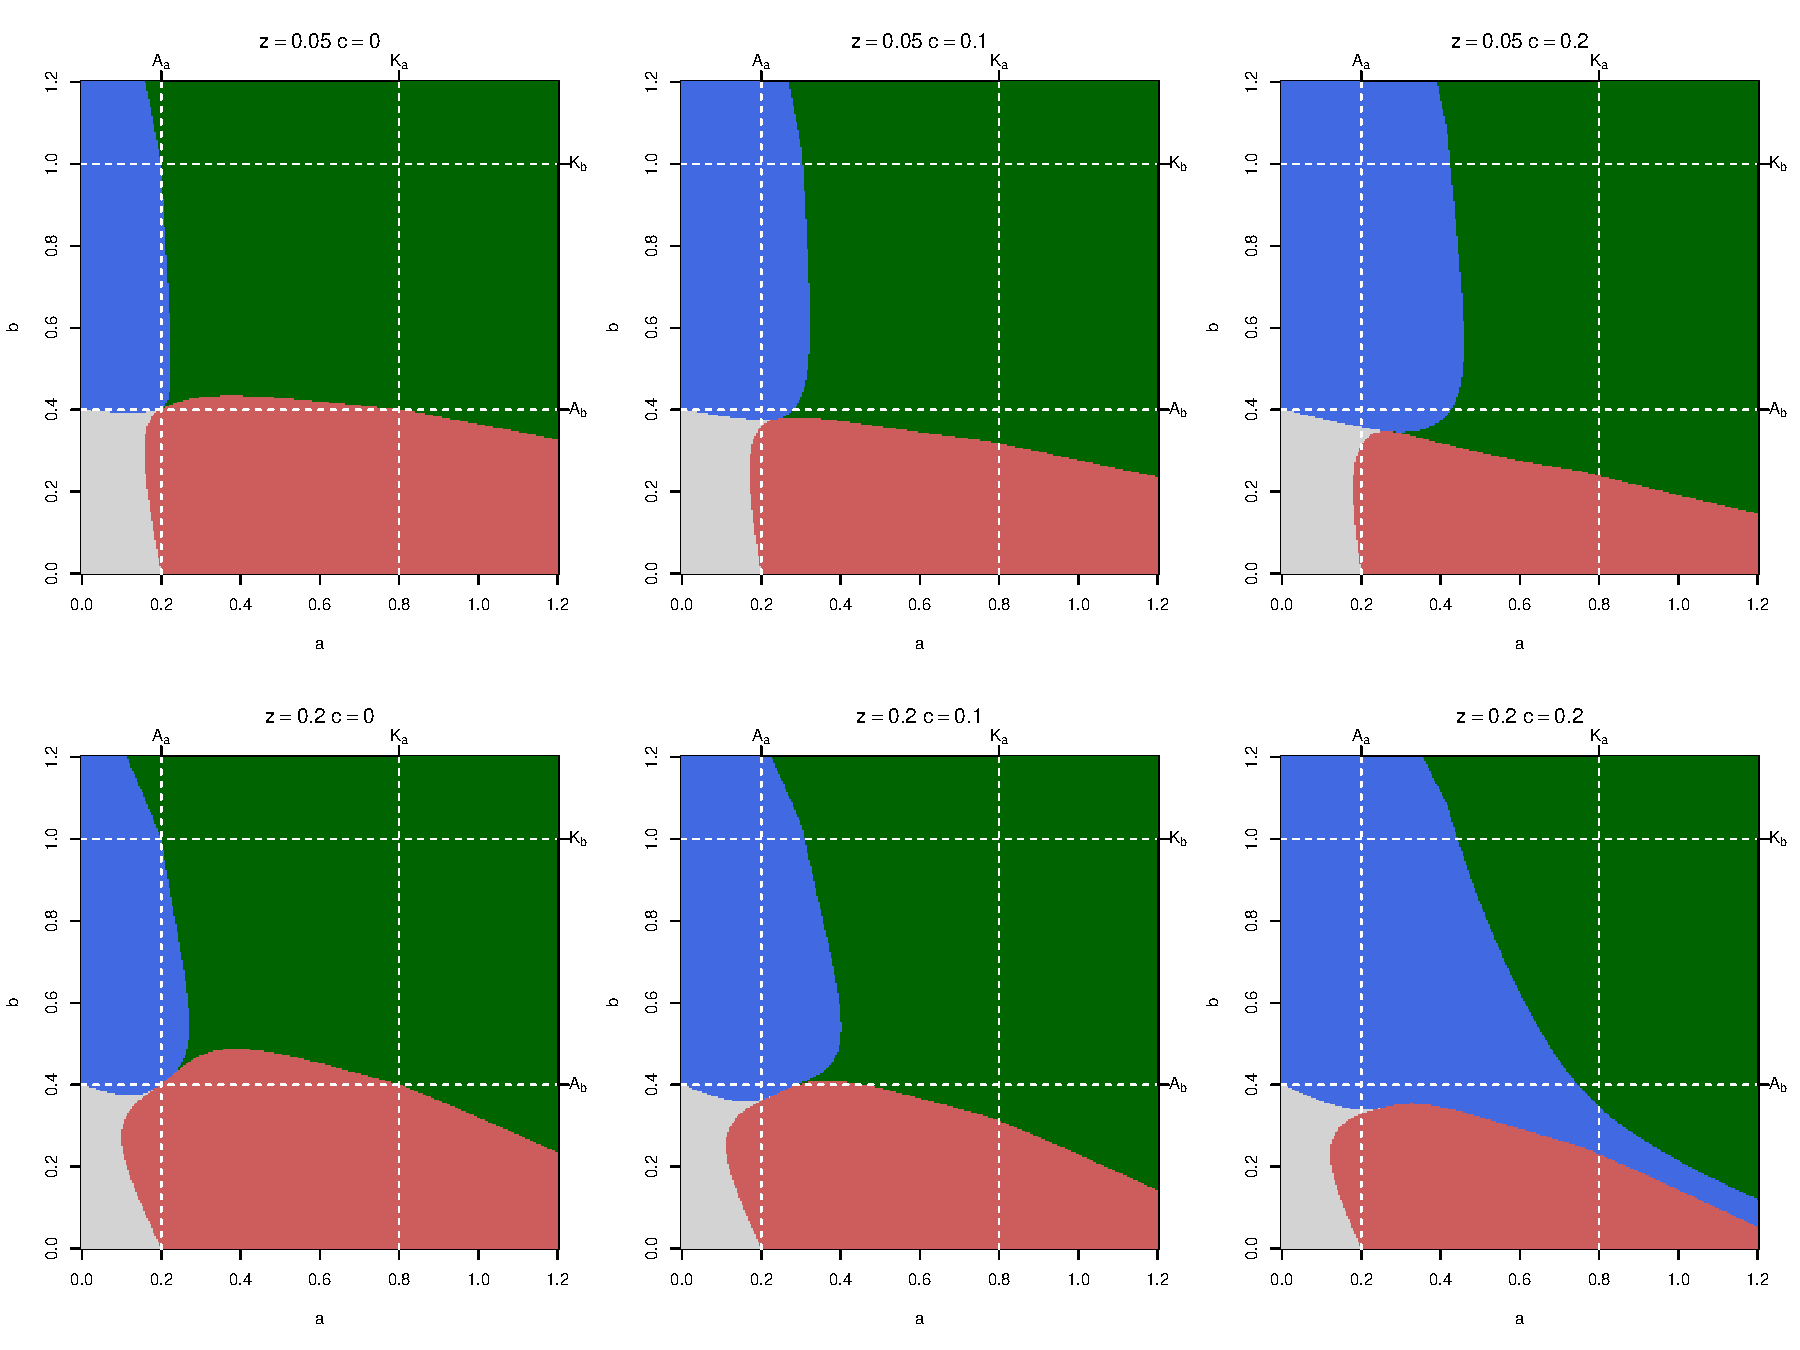
\includegraphics[width=\textwidth]{./figures/figure7}
  \caption{The impact of competition on the basins of attraction for the different equilibria. The Parameters used are $z=0.05$ (up) and $z=0.2$ (bottom) for social learning, and $c=0$ (left), $c=0.1$ (center) and $c=0.2$ (right) for competition.}
    \label{fig:competition}
\end{figure*}

\section{Discussion}

Our analysis examined the impact of direct and inverse density dependence in payoff-based social learning strategies. The results showed that Allee effect lead to the emergence of both positive and negative feedback mechanisms, and can generate a wide range of patterns where small changes in the initial conditions can deeply affect the evolutionary trajectories of the system. Our theoretical model indicated that social learning can in fact alter the basins of attraction of stable nodes, leading to different dynamics and equilibria from the very same initial conditions. If there is no reliance on social learning, the critical density separates the ultimate equilibrium of the system: if the initial condition is below this threshold the variant is destined to go extinct, whilst if it is above this value will eventually reach carrying capacity. When social learning is present this boundary shifts; variants can survive even if its initial condition is below critical density and equally can reach extinction even if above this threshold. This scenario is also observed when the two variants are not independent but are in direct competition. In this case, social learning can further enhance the advantage of one variant over the other. 

When the reliance on social learning is comparatively high, and the two variants have a substantial overlap in their range of positive payoff densities (i.e. they share similar critical densities and carrying capacities), the system does not always reach an stable equilibrium, but can instead exhibit cyclical fluctuations. In other words the impact of social learning is not absorbed by the system, and instead a negative feedback process leads to continuous switch from one variant to the other. 

The implications of our model can provide some insights in the evolutionary history of cultural traits exhibiting density dependence. Perhaps the most notable example is the spread of keystone innovations in subsistence strategies which led to the adoption of variants enabling larger carrying capacity, often at the cost of higher critical densities. The spread of behavioural traits such as the know-how of the domestication process~\citep{barker2006}, the use of new subsistence tools~\citep{petraglia_population_2009} and processing techniques~\citep{molleson1993}, as well as the inclusion/exclusion and extensification/intensification of different prey species are just some of the most notable examples. In many of these examples the initial spread of the innovation generated a positive feedback process, either through enhanced possibility of direct cooperation, or some form of mutual facilitation often indirectly emerging from positive niche construction. At the same time, ethnographic and archaeological evidence show how many instances of critical transitions where not smooth, often leading to the coexistence of alternative strategies as well as episodes of a return to previously abandoned cultural traits (see Day and Walter \citeyear{day_and_walter_1989} for similar insights in economics). Several ethnographic examples showcase small-scale societies alternating between different subsistence modes over a comparatively brief period of time \citep{layton1991,mace_1993,oota_et_al_2005}, while increasing archaeological evidence suggests that the transition from hunting-gathering to farming was not unidirectional, but with instances of temporary reversions \citep{rowley2001,stevens_fuller_2012}. Formal cross-cultural analysis of these episodes are still rare (but see Ullah et al. \citeyear{ullah_etal_2015}) but the insights of our model suggests that different levels of reliance on social learning could alone portray some of the evolutionary trajectories observed in these systems. 

\section{References}

\bibliographystyle{elsarticle-harv}
\bibliography{references}


\end{document}

